\chapter{Analysis of the Current VCA-Based System}

\section{Overview of the Current VCA System}
This section provides an overview of the existing Voice Coil Actuator (VCA)-based setup. The System consists of seven main parts. 

\begin{itemize}
    \item Spring frame (Minimizing the loss of vertical motion transmitted to the node)
    \item Magnet Housing (fixed Magnetic field is always formed)
    \item Bobbin Coil (Magnetic field is formed only when current flows)
    \item Node (Transmitting vertical motion directly to the human body as sound and vibration)
    \item Node screw (fixes the node to the bobbin coil)
    \item Rubber frame (Suppresses vibration from the body from being transmitted to the outside world)
    \item Connection PCB (Take the analog signal from the AMP and apply it to the bobbin coil)
\end{itemize}

\begin{figure}[H]
    \centering
    \includegraphics[width=0.62\textwidth]{img/coil.png}
    \caption[coil model]{coil model}
    \label{fig:CoilModel}
\end{figure}

\begin{figure}[ht]
    \centering
    \begin{subfigure}[b]{0.45\textwidth}
    \includegraphics[width=\textwidth]{img/B_Vektor_Iso.jpg}
    \caption{}
    \label{subfig:B_Vektor_Iso}
    \end{subfigure}
    \hfill
    \begin{subfigure}[b]{0.45\textwidth}
    \includegraphics[width=\textwidth]{img/B_Vektor_Top.jpg}
    \caption{}
    \label{subfig:B_Vektor_Top}
    \end{subfigure}
    \vspace{0.1cm}
    \caption{Ansys simulation of the B-field in the Magnet Housing (a) VCA in iso view (b) VCA in top view}
    \label{fig:B_Vektor}
\end{figure}


\begin{figure}[H]
    \centering
    \includegraphics[width=0.62\textwidth]{img/Force Plot 1.png}
    \caption[Force Plot]{Force Plot}
    \label{fig:ForcePlot}
\end{figure}



\section{Dynamic Behavior: Frequency Measurement}

\subsection{Objective}

\subsection{Measurement Setup}


\subsection{Results \& Interpretation}

\begin{figure}[H]
    \centering
    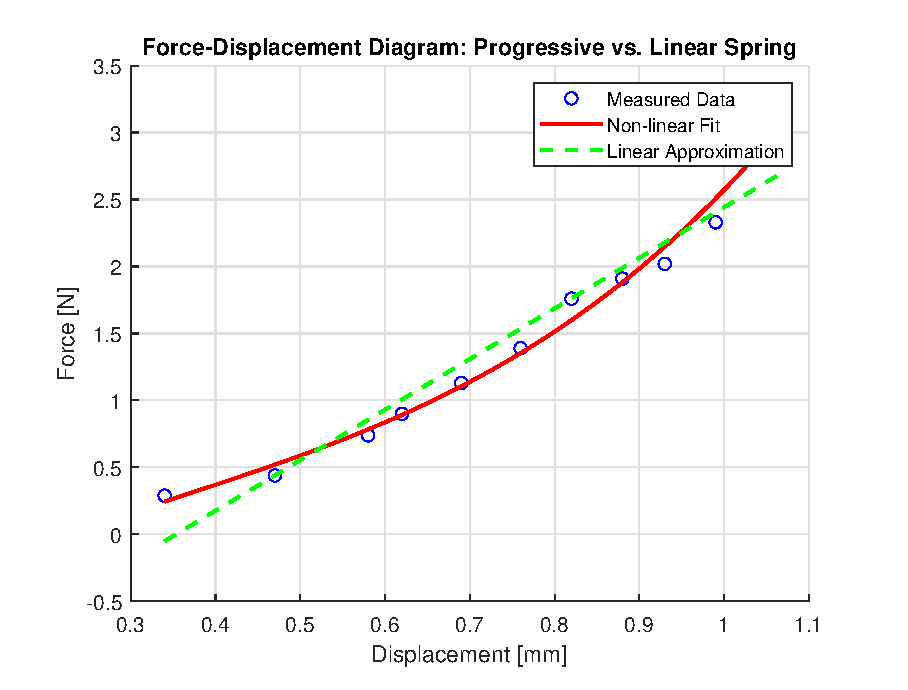
\includegraphics[width=0.62\textwidth]{img/SpringTest.eps}
    \caption[SpringTest]{SpringTest}
    \label{fig:SpringTest}
\end{figure}


\section{Limitations and Identified Challenges}
